
%!TEX TS-program = xelatex
%!TEX encoding = UTF-8 Unicode

\documentclass[11pt,twoside,a4paper]{book}

	%Establecemos el tamaño de la hoja a a4 y el tamaño de los márgenes izquierdo y derecho al mínimo
	\usepackage[a4paper,hmargin={2cm,2cm},vmargin={3cm,3cm}]{geometry} 

	% Paquetes para uso de matemáticas
	\usepackage{amssymb}

	% Para poder usar \boldsymbol que nos permite poner negrita a expresiones ``matemáticas'' en modo matemático.
	\usepackage{amsmath}

	% Paquete para introducir símbolos dingbats
	\usepackage{pifont}

	% Paquete para usar imágenes jpg y png
	\usepackage{graphicx}

	% Paquete para poder usar colores
	\usepackage{xcolor}
	
	% Paquete para soportar silabeo en castellano
	\usepackage[spanish]{babel}

	% Activate to begin paragraphs with an empty line rather than an indent
	\usepackage[parfill]{parskip}

	\usepackage{pifont}

	% Identar el comienzo de cada parrafo
	\usepackage{indentfirst}

	% Paquete para poder centrar verticalmente las columnas de las tablas
	\usepackage{array}
	\usepackage{tabularx}
	\usepackage{multirow}
		
	% Permite usar enlaces (por ejemplo desde la tabla de contenidos)
	\usepackage{hyperref}
 
    \hypersetup{
        colorlinks,%
        citecolor=black,%
        filecolor=black,%
        linkcolor=black,%
        urlcolor=black
    }

	% Permite cambiar el títulos de las páginas
	\usepackage{fancyhdr}
	
	% Personalización de las cabeceras con fancyhdr
    \fancyhead{} % clear all header fields 
    \fancyfoot{} % clear all footer fields 
    \fancyhead[RE,LO]{\bfseries Compilación 1 }
    \fancyhead[RO,LE]{\small{\bfseries Jon Ander Hernández, Alberto Alonso y Gorka Blanco (JAG)}}
    \fancyfoot[LE,RO]{\thepage} 
    \fancyfoot[LO,CE]{} 
    \fancyfoot[CO,RE]{} 
    \renewcommand{\headrulewidth}{0.4pt} 
    \renewcommand{\footrulewidth}{0.4pt} 

    \pagestyle{fancy}

    \fancypagestyle{plain}{% 
    \fancyhead{} % clear all header fields 
    \fancyfoot{} % clear all footer fields 
    \fancyhead[RE,LO]{\bfseries Compilación 1 }
    \fancyhead[RO,LE]{\small{\bfseries Jon Ander Hernández, Alberto Alonso y Gorka Blanco (JAG)}}
    \fancyfoot[LE,RO]{\thepage} 
    \fancyfoot[LO,CE]{} 
    \fancyfoot[CO,RE]{} 
    \renewcommand{\headrulewidth}{0.4pt} 
    \renewcommand{\footrulewidth}{0.4pt}}


	% Podemos cambiar las fuentes por defecto Serif, San Serif, y Mono en _XeTeX_ y usar fuentes OpenType y AAT.
	\usepackage{fontspec,xltxtra,xunicode}
	\defaultfontfeatures{Mapping=tex-text}
	%\setromanfont[Mapping=tex-text]{Hoefler Text}
	%\setsansfont[Scale=MatchLowercase,Mapping=tex-text]{Gill Sans}
	%\setmonofont[Scale=MatchLowercase]{Andale Mono}

	% Paquete para poder incluir código fuente
	\usepackage[formats]{listings}

    % Establecemos los valores por defecto de Listings
	\lstset{
		language={C++},                              % Lenguaje por defecto
		%
		% estilos
		keywordstyle=\bfseries\ttfamily\color[rgb]{.8,.1,.2},	% estilos de palabras clave, identificadores, etc...
		identifierstyle=\ttfamily,
		commentstyle=\color[rgb]{0.1,0.5,0.1},			 
		stringstyle=\ttfamily\color[rgb]{0.2,0.2,.7},			
		basicstyle=\footnotesize,                    % the size of the fonts used for the code 		%
		% espacios
		showspaces=false,                            % show spaces adding particular underscores 
		showstringspaces=false,                      % underline spaces within strings 
		showtabs=false, 							% show tabs within strings through particular underscores 
		tabsize=6,									% sets default tab-size to 2 spaces
		%
		% cuadro
		backgroundcolor=\color{white}, 				% sets background color (needs package) 
		frame=single, 								% adds a frame around the code
		rulecolor=\color[rgb]{1,.3,.3},					% set the frame's color. 
		captionpos=b, 								% sets the caption-position to bottom 
		%
		% line breaking
		breaklines=true, 							% sets automatic line breaking 
		breakatwhitespace=false, 					% automatic breaks happen at whitespace 
		prebreak = \raisebox{0ex}[0ex][0ex]{\ensuremath{\hookleftarrow}} % Nos dibuja una flecha ``guay'' cuando el código no entra en una linea
	}

% Reescribimos algunas macros para cambiar algunos parámetros

	% Establecemos el interlineado a 1.2
	\renewcommand{\baselinestretch}{1.2}

	\newcommand{\ter}[1]{
		\textbf{#1}
	}

	\newcommand{\sem}[1]{\textcolor{red}{ $ \left \{ 
		\begin{tabular*}{0.7\textwidth}{lll}
		#1
		\end{tabular*} \right \} $
	}}
	
	\newcommand{\ind}{\hspace{1em}}
	
	\newcommand{\espacio}{
		\\ \\
	}
	

\author{ \href{mailto:jahernandez002@ikasle.ehu.es}{Jon Ander Hernández} \and 
         \href{mailto:aalonso065@ikasle.ehu.es}{Alberto Alonso} \and
         \href{mailto:gblanco002@ikasle.ehu.es}{Gorka Blanco Gutierrez} \\[.5em] \and
         %
         \small\href{mailto:jahernandez002@ikasle.ehu.es}{jahernandez002@ikasle.ehu.es} \and 
         \small\href{mailto:aalonso065@ikasle.ehu.es}{aalonso065@ikasle.ehu.es} \and
         \small\href{mailto:gblanco002@ikasle.ehu.es}{gblanco002@ikasle.ehu.es} \\[1em] }
         
         
\title{%
	% Creamos un entorno de centrado
	\begin{centering}
		% Establecemos la fuente
		\fontspec[Ligatures={Common},Color=000000]{Hoefler Text}\fontsize{50pt}{50pt}\selectfont 
		% El título en grande
		Compilación I. 
	\end{centering}
	%
	\newline \Huge{Entrega Final.}
	%
	% Dejamos un hueco flexible, de modo que los autores bajen hasta la parte de abajo del documento
	\vfill
}



\begin{document}

    % Para que fancyhdr no incluya un pie ni una cabecera en la portada
    \thispagestyle{empty}

    % Creamos la portada
    \maketitle

    \thispagestyle{empty}
    
    \cleardoublepage
    
    
    % Creamos la tabla de contenidos
    \tableofcontents

\part{Analizador léxico}

	
\part{Analizador léxico}


\chapter{Análisis léxico: Especificación de los tokens}
    
    \section{Espacios}
    
        \subsection{Descripción}
        
            Usamos este tipo de Token para representar el conjunto de espacios, aunque este Token será ignorado desde el nivel sintáctico.
        
            A la hora de interpretar el documento, emplearemos 2 autómatas. Uno para interpretar los espacios convencionales, y otro para interpretar los saltos de linea, ya que a medida que vamos leyendo el documento iremos contando el número linea para reportarlo en caso de error.
        
        \subsection{Atributos}
        
            Ninguno
            
	    \subsection{Espacios normales}
     
            \subsubsection{Expresión regular}
                \begin{lstlisting}[language=Perl]
[\ \t]+
                \end{lstlisting}

            \subsubsection{Autómata}
            
                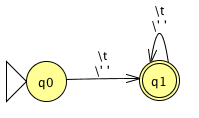
\includegraphics[scale=.7]{../Design/jflap/Espacio.png}
                
        \subsection{Saltos de linea}
        
            \subsubsection{Expresión regular}
            
                \begin{lstlisting}[language=Perl]
\n|\r|\r\n
                \end{lstlisting}
                
            \subsubsection{Autómata}
         
                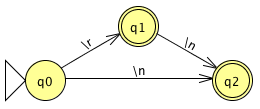
\includegraphics[scale=.7]{../Design/jflap/Salto_de_linea.png}
            
        \subsection{Notas}
        
            \begin{itemize}
            
                \item Con el método NextToken de la clase Tokenizer, podemos indicar si queremos filtrar los espacios y/o los saltos de linea.
            
            \end{itemize}
            
            \hfill
            \clearpage
            
            
            
    \section{Separadores}
    
        \subsection{Descripción}
        
            Usamos este tipo de Token para representar el conjunto de separadores :
            
            \begin{itemize}
                \item Paréntesis. Empleados para indicar los argumentos de los procedimientos.
                \item Punto y coma. Empleados para separar las instrucciones.
                \item Dos puntos. Para separar el tipo de los identificadores en las declaraciones de variables.
                \item Coma. Para separar los argumentos de los procedimientos, y los identificadores en las declaraciones de las variables.
            \end{itemize}
            
        \subsection{Expresión regular}
            
             \begin{lstlisting}[language=Perl]
[(),:;]
             \end{lstlisting}


        \subsection{Autómata}
            
	        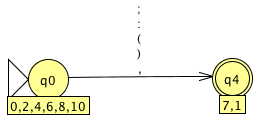
\includegraphics[scale=.7]{../Design/jflap/Separador.png}
	        
        \subsection{Atributos}
        
            \begin{itemize}
                \item Número de linea
                \item Número de columna
                \item Valor.
            \end{itemize}
            
            \hfill
            \clearpage
            
     
    
    \section{Comentario}
    
        \subsection{Descripción}
        
            Usamos este tipo de Token para representar los comentarios, aunque este Token será ignorado desde el nivel sintáctico.
            
            Los comentarios pueden ser multilinea, y aceptan cualquier contenido en su interior hasta encontrar el cierre del comentario.
        
        \subsection{Expresión regular}
            
             \begin{lstlisting}[language=Perl]
\/\*([^*]|(\*+[^*\/]))*\*+\/
             \end{lstlisting}
            
        \subsection{Autómata}
        
            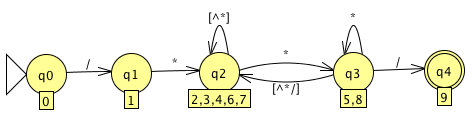
\includegraphics[scale=.7]{../Design/jflap/Comentario.png}

        \subsection{Atributos}
        
            \begin{itemize}
                \item Número de linea.
                \item Número de columna.
                \item Valor.
            \end{itemize}
            
            \hfill
            \clearpage
            


	\section{Identificador}

        \subsubsection{Descripción}
        
            Usamos este tipo de Token para representar un identificador.
            
            Los identificadores son de tipo Ada con subrayado: Empiezan por carácter alfabético, puede contener caracteres alfanuméricos o guión bajo, pero no puede comenzar ni terminar con un guión bajo ni puede contener dos guiones bajos seguidos.
            
        \subsection{Expresión regular}

            \begin{lstlisting}[language=Perl]
[a-zA-Z](_?[a-zA-Z0-9])*
            \end{lstlisting}

        \subsection{Autómata}
        
            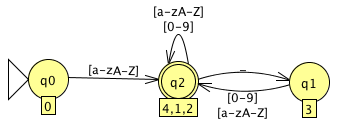
\includegraphics[scale=.7]{../Design/jflap/Identificador.png}

        \subsection{Atributos}
        
            \begin{itemize}
                \item Número de linea.
                \item Número de columna.
                \item Valor.
            \end{itemize}

            \hfill
            \clearpage
            



	\section{Constante entera}
    
        \subsection{Descripción}
        
            Usamos este tipo de Token para representar las constantes enteras.
        
        \subsection{Expresion regular}
        
            \begin{lstlisting}[language=Perl]
[0-9]+
            \end{lstlisting}

        \subsection{Autómata}
        
	        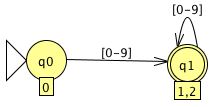
\includegraphics[scale=.7]{../Design/jflap/Constante_entera.png}

        \subsection{Atributos}
        
            \begin{itemize}
                \item Número de linea.
                \item Número de columna.
                \item Valor.
            \end{itemize}

            \hfill
            \clearpage
            
            
            
            
	\section{Constante real}

        \subsection{Descripción}

            Usamos este tipo de Token para representar las constantes reales, es decir números reales con decimales y exponencial.

        \subsection{Expresion regular}

            \begin{lstlisting}[language=Perl]
[0-9]+\.[0-9]+([eE][+\-]?[0-9]+)?
            \end{lstlisting}

        \subsection{Autómata}

            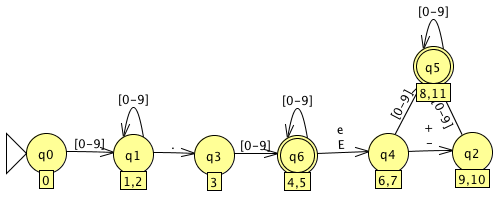
\includegraphics[scale=.7]{../Design/jflap/Constante_real.png}

        \subsection{Atributos}

            \begin{itemize}
                \item Número de linea.
                \item Número de columna.
                \item Valor.
            \end{itemize}

            \hfill
            \clearpage




	\section{Operadores}

        \subsection{Descripción}
        
            Usamos este tipo de Token para representar los operadores :
            
            \begin{itemize}
            
                \item Aritméticos
                \item Relacionales
                \item Operador asignación
                
            \end{itemize}
        
        \subsection{Operadores aritméticos}
        
            \begin{lstlisting}[language=Perl]
[+-*/]
            \end{lstlisting}

        \subsection{Operadores relacionales}

            \begin{lstlisting}[language=Perl]
[<>]|[/<>=]=
            \end{lstlisting}
            
        \subsection{Operador asignación}

            \begin{lstlisting}[language=Perl]
=
            \end{lstlisting}

        \subsection{Todos los operadores}

            \begin{lstlisting}[language=Perl]
[+-*/]|[<>]|[/<>=]=|=
            \end{lstlisting}

        \subsection{Autómata Operadores}

            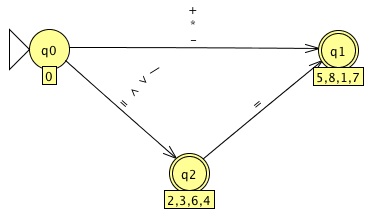
\includegraphics[scale=.7]{../Design/jflap/Operadores.png}

        \subsection{Atributos}

            \begin{itemize}
                \item Número de linea.
                \item Número de columna.
                \item Valor.
            \end{itemize}

            \hfill
            \clearpage



\section{Autómata competo unificado}

         \hspace{-7.8em}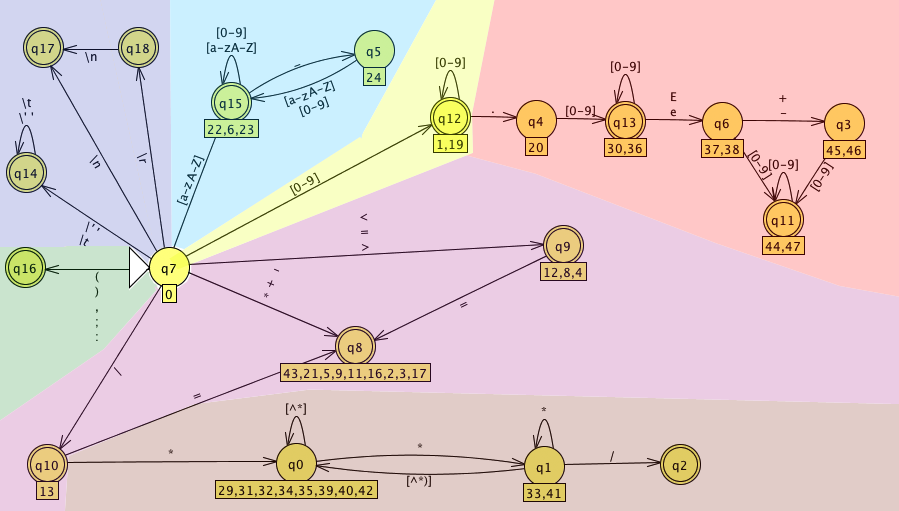
\includegraphics[scale=.61]{../Design/jflap/automata.png}

            \hfill
            \clearpage


 
\section{Listado de palabras reservadas}
    
        \subsection{Descripción}
        
        La palabras reservadas son identificadores reservados con un significado especial en nuestro lenguaje.
        
        \begin{itemize}
             \item programa
             \item procedimiento
             \item entrada
             \item salida
             \item si
             \item entonces
             \item fin
             \item hacer
             \item mientras
             \item salir
             \item get
             \item put\_line
       \end{itemize}

       \hfill
       \clearpage





	
\chapter{Casos de prueba. Entrada y salida obtenida}
	
	
\section{Programa lexicamente completo}
	
    \subsection{Programa}
	    
        \lstinputlisting{../ejemplos/ejem0.dat}
	
   \subsection{Salida}
	    
        \lstinputlisting[basicstyle=\small]{../ejemplos/ejem0_salida.txt}

    % Rellena el resto de la página, y termina la página actúal
    \hfill
    \clearpage

	

\section{Programa con comentarios erróneos}

    \subsection{Programa}
	    
        \lstinputlisting{../ejemplos/ejem1.dat}
	
   \subsection{Salida}
	    
        \lstinputlisting{../ejemplos/ejem1_salida.txt}

    % Rellena el resto de la página, y termina la página actúal
    \hfill
    \clearpage



\section{Programa con identificadores inválidos}

    \subsection{Programa}
	    
        \lstinputlisting{../ejemplos/ejem2.dat}
	
   \subsection{Salida}
	    
        \lstinputlisting{../ejemplos/ejem2_salida.txt}

    % Rellena el resto de la página, y termina la página actúal
    \hfill
    \clearpage




\section{Programa con constantes enteras erróneas}

    \subsection{Programa}
	    
        \lstinputlisting{../ejemplos/ejem3.dat}
	
   \subsection{Salida}
	    
        \lstinputlisting{../ejemplos/ejem3_salida.txt}

    % Rellena el resto de la página, y termina la página actúal
    \hfill
    \clearpage

	
	
\chapter{Mejoras}

\begin{itemize}

    \item Compilable en Windows, Mac OS X y Linux, mediante un Makefile generado con netbeans.

    \item Hemos implementado la práctica en C++ desde cero.
    
    \item La tabla de clases de caracteres incluye una columna Unknown que nos sirve para aceptar cualquier tipo de entrada en algunas transiciones. Como por ejemplo en los comentarios, que permite incluir cualquier carácter hasta llegar al final del comentario.
    
    \item Triggers. Los estados pueden contener una rutina que es ejecutada cuando se llega a dicho estado. Utilizamos esta funcionalidad en los comentarios para registrar los saltos de linea en los comentarios multilinea.
    
    \item La función NextToken del Tokenizer nos permite parametrizar si queremos filtrar los espacios y los saltos de linea.
    
    \item Leemos los ficheros mediante una abstracción que realiza buffering.
    
    \item Documentación escrita en \LaTeX.
    
\end{itemize}


\part{Analizador sintáctico y semántico}
	
	\chapter{Gramática}

\small
\begin{tabular}{r c p{.72\textwidth}}
	
	programa 		&$\longrightarrow$	& \ter{programa} \ter{id} \\
					&				 	& \sem{ ADD\_INST('prog ' || ID.value); } \\
					&					& declaraciones \\
					&					& decl\_de\_subprogs \\
					&					& \ter{comienzo} \\
					&					& lista\_de\_sentencias\_prima \\
					&					& \ter{fin} \ter{;} \\
					&					& \sem{ ADD\_INST\_inst('halt'); } \\

	\espacio
	
	declaraciones 	&$\longrightarrow$ 	& \ter{variables} lista\_de\_ident \ter{:} tipo \ter{;} \\
					&					& \footnotesize\sem{ if ( IS\_INTEGER( t.tipo) || IS\_REAL(t.tipo) || IS\_BOOLEAN(t.tipo) ) \\
												\{ \\
												\ind FOREACH( lista\_de\_ident.ids AS ident) \\
												\ind\ind ADD\_INST( TYPE\_OF(tipo.tipo) || " " || ident); \\
												\} \\
												else if ( IS\_ARRAY(t.tipo) ) \\
												\ind FOREACH( lista\_de\_ident.ids AS ident) \\
												\ind\ind ADD\_INST( ``array'' || TYPE\_OF(ARRAY\_CONTENT(t.tipo)) || `` '' \\
												\ind\ind\ind\ind\ind\ind\ind\ind || ident || ``,'' || ARRAY\_SIZE(t.tipo) ); \\
										  } \\
					&					& declaraciones \\
										
					& | 					& $\xi$ \\



	\espacio

	declaraciones 	&$\longrightarrow$ 	& \ter{variables} lista\_de\_ident \ter{:} tipo \ter{;} \\
					&					&         \begin{lstlisting}[caption={Trigger para contar lineas en un comentario multilinea}]
void CTokenizer::CheckMultilineComment ( unsigned char c )
{
    static bool bLastCharWasCR = false;

    switch ( c )
    {
        case '\r':
            bLastCharWasCR = true;
            ++m_uiLine;
            m_uiCol = 0;
            break;
        case '\n':
            m_uiCol = 0;
            if ( bLastCharWasCR == true )
            {
                bLastCharWasCR = false;
            }
            else
            {
                ++m_uiLine;
            }
            break;
    }
}
        \end{lstlisting} \\
					&					& declaraciones \\
										
					& | 					& $\xi$ \\

	\espacio
	
	lista\_de\_ident	&$\longrightarrow$	& \ter{id} resto\_lista\_id \\
					&					& \sem{lista\_de\_ident.ids := JOIN( & INIT\_LIST(id.value), \\
																			& resto\_lista\_ident.ids); } \\

\end{tabular}


\small
\begin{tabular}{r c p{.72\textwidth}}
	
	resto\_lista\_ident 	& $\longrightarrow$ 	& \ter{,} \ter{id} resto\_lista\_id \\
						&					& \sem{ resto\_lista\_ident.ids := JOIN(	& INIT\_LIST(id.value) , \\
																					& resto\_lista\_id.ids); } \\
																			
						& | 					& $\xi$ \\
						&					& \sem{ resto\_lista\_ident.ids := EMPTY\_LIST(); } \\

	\espacio
	
	tipo 			& $\longrightarrow$ 	& entero \\
					&					& \sem{ tipo.tipo := 'int'} \\
					
					& | 					& real \\
					&					& \sem{ tipo.tipo := 'real'} \\
					
					& | 					& booleano \\
					&					& \sem{tipo.tipo := 'booleano'} \\

					& | 					& \ter{array} \ter{[} lista\_de\_enteros \ter{]} \ter{de} tipo \\
					&					& \sem{ tipo.tipo := NEW\_ARRAY\_TYPE(lista\_de\_enteros, tipo); } \\
					
	\espacio	
	

	
	lista\_de\_enteros	& $\longrightarrow$ 	& entero resto\_lista\_enteros \\
						&					& \sem{ lista\_de\_enteros := JOIN(INIT\_LIST(entero), resto\_de\_enteros.ints); } \\
					
	\espacio

	resto\_de\_enteros	& $\longrightarrow$ 	& entero resto\_lista\_enteros\textsubscript{1} \\
						&					& \sem{ resto\_de\_enteros := JOIN(	& INIT\_LIST(entero), \\
																				& resto\_de\_enteros\textsubscript{1}.ints); } \\
						& | 					& $\xi$ \\
						&					& \sem{ resto\_de\_enteros := EMPTY\_LIST } \\
					
	\espacio
	
	decl\_de\_subprogs 		& $\longrightarrow$ 	& decl\_de\_procedimiento decl\_de\_subprogs \\
							& |					& decl\_de\_funcion decl\_de\_subprogs \\
							& | 					& $\xi$ \\

\end{tabular}

\small
\begin{tabular}{r c p{.72\textwidth}}

	decl\_de\_procedimiento 	& $\longrightarrow$ 	& \sem{ ST\_PUSH(); } \\
							&					& cabecera\_procedimiento declaraciones \\
							&					& \ter{comienzo} lista\_de\_sentencias\_prima \ter{fin} \\
							&					& \sem{ ADD\_INST(``finproc''); } \\
							&					& \ter{;} \\
							&					& \sem{ ST\_POP(); } \\
							
							
	\espacio
	
	decl\_de\_function	 	& $\longrightarrow$ 	& \sem{ ST\_PUSH(); } \\
							&					& cabecera\_funcion declaraciones \\
							&					& \ter{comienzo} lista\_de\_sentencias\_prima \ter{retornar} expresion \\
							&					& \sem{ if ( & cabecera\_funcion.tipo == expresion.tipo) \{ \\
																& ADD\_INST( ``ret '' || expresion.nombre ); \\
																& ADD\_INST( ``finfunc''); \\
														\} else & \{ \\
																& ERROR( "Function return type mismatch" ); \\
														\} } \\
							&					& \ter{fin} \\
							&					& \ter{;} \\
							&					& \sem{ ST\_POP(); } \\

	\espacio
	
	cabecera	\_procedimiento 	&$\longrightarrow$	& \ter{procedimiento} \ter{id} \\
							& 					& \sem{'proc ' || id.value } \\
							&					& argumentos \\

	\espacio

	cabecera	\_funcion	 	&$\longrightarrow$	& \ter{funcion} \ter{id} \\
							& 					& \sem{'func ' || id.value } \\
							&					& argumentos \ter{retorna} tipo \\
							&					& \sem{cabecera	\_funcion := tipo.tipo } \\
	
	\espacio
		
	argumentos 		&$\longrightarrow$ 	& \ter{(} lista\_de\_param \ter{)} \\
					& | 					& $\xi$ \\
							
\end{tabular}


\small
\begin{tabular}{r c p{.72\textwidth}}
	lista\_de\_param &$\longrightarrow$  	& lista\_de\_ident \ter{:} clase\_par tipo \\
					&					& \sem{ FOREACH(	lista\_de\_ident.ids as id) \{ \\
												\ind ADD\_INST( clase\_par.clase || ``\_'' || TYPE\_OF(tipo.tipo) || `` '' || id); \\
										\} \\
										} \\
					&					& resto\_lis\_de\_param \\
					
	\espacio
	
	resto\_lis\_de\_param 	&$\longrightarrow$ 	& \ter{;} lista\_de\_ident \ter{:} clase\_par tipo \\
							&					& \sem{ FOREACH(	lista\_de\_ident.ids as id) \{ \\
														\ind ADD\_INST(clase\_par.clase || ``\_'' || TYPE\_OF(tipo.tipo) || `` '' || id); \\
												\} } \\
							&					& resto\_lis\_de\_param \\
							& |					& $\xi$ \\

	\espacio


	clase\_par 		& $\longrightarrow$		& entrada clase\_par' \\
					&						& \sem{clase\_par.clase := clase\_par'.clase; } \\ 
					& | 						& salida \\
					&						& \sem{clase\_par := 'ref'; } \\
	
	\espacio
	
	clase\_par' 		& $\longrightarrow$		& salida \\
					&						& \sem{clase\_par := 'ref'; } \\ 
					& | 						& $\xi$ \\
					&						& \sem{clase\_par := 'val'; } \\
					
	\espacio

	lista\_de\_sentencias' 	& $\longrightarrow$ 	& \sem{ lista\_de\_sentencias.hinloop := false; } \\
							& 					& lista\_de\_sentencias \\

	\espacio

\end{tabular}

\small
\begin{tabular}{r c p{.72\textwidth}}
	lista\_de\_sentencias 	& $\longrightarrow$ 	& \sem{sentencia.hinloop:=lista\_de\_sentencias.hinloop} \\
							& 					& sentencia \ter{;} \\
							&					& \sem{ lista\_de\_sentencia\textsubscript{1}.hinloop:=lista\_de\_sentencias.hinloop; } \\
							&					& lista\_de\_sentencias\textsubscript{1} \\
							&					& \sem{ lista\_de\_sentencias.salir\_si := unir( 	& sentencia.salir\_si, \\
																								& lista\_de\_sentencia\textsubscript{1}.salir\_si ) } \\
							& | 					& $\xi$ \\
							&					& \sem{lista\_de\_sentencias.salir\_si := lista\_vacia() } \\

\end{tabular}

	\chapter{Demostración LL1}

\small
\begin{tabular}{| l | p{.27\textwidth} | p{.27\textwidth} | c | c | } \hline

\textbf{Regla} & \textbf{Primero} & \textbf{Siguiente} & {\scriptsize Cond1} & {\scriptsize Cond2} \\ \hline


programa						& programa
             				& \# & \ding{52} & \ding{52} \\ \hline

declaraciones				& variables $\xi$ 
							& procedimiento funcion comienzo & \ding{52} & \ding{52} \\ \hline

lista\_de\_ident				& IDENTIFIER
							& :	 & \ding{52} & \ding{52} \\ \hline

resto\_lista\_ident			& , $\xi$
							& : & \ding{52} & \ding{52} \\ \hline

tipo							& entero real booleano array
							& ; variables comienzo ) & \ding{52} & \ding{52} \\ \hline

lista\_de\_enteros			& INTEGER
							& ] & \ding{52} & \ding{52} \\ \hline

resto\_lista\_enteros		& ,  $\xi$
							& ] & \ding{52} & \ding{52} \\ \hline

decl\_de\_subprogs			& procedimiento funcion $\xi$
							& comienzo & \ding{52} & \ding{52} \\ \hline

decl\_de\_procedimiento		& procedimiento
							& procedimiento funcion comienzo & \ding{52} & \ding{52} \\ \hline

decl\_de\_funcion			& funcion
							& procedimiento funcion comienzo & \ding{52} & \ding{52} \\ \hline

cabecera\_procedimiento		& procedimiento
							& variables comienzo & \ding{52} & \ding{52} \\ \hline

cabecera\_funcion			& funcion
							& variables comienzo & \ding{52} & \ding{52} \\ \hline

argumentos					& ( $\xi$
							& variables comienzo retorna & \ding{52} & \ding{52} \\ \hline

lista\_de\_param				& IDENTIFIER
							& ) & \ding{52} & \ding{52} \\ \hline

resto\_lis\_de\_param		& ;  $\xi$
							& ) & \ding{52} & \ding{52} \\ \hline

clase\_param					& entrada salida
							& entero real booleano array & \ding{52} & \ding{52} \\ \hline

clase\_param'				& salida 	$\xi$
							& entero real booleano array & \ding{52} & \ding{52} \\ \hline

lista\_de\_sentencias'		& IDENTIFIER si hacer salir get put\_line $\xi$
							& fin retorna & \ding{52} & \ding{52} \\ \hline

lista\_de\_sentencias		& IDENTIFIER si hacer salir get put\_line $\xi$
							& fin  retorna mientras & \ding{52} & \ding{52} \\ \hline


sentencia					& IDENTIFIER si hacer salir get put\_line
							& IDENTIFIER si hacer salir get put\_line fin retorna mientras & \ding{52} & \ding{52} \\ \hline

id\_o\_array					& [ $\xi$
							& ) & \ding{52} & \ding{52} \\ \hline

asignacion\_o\_llamada		& =  [  (
							& ;  ) & \ding{52} & \ding{52} \\ \hline

acceso\_a\_array				& [
							& = * / + - < > <= >= == /= and  or  entonces  fin  ;  )  ] , & \ding{52} & \ding{52} \\ \hline

\end{tabular}

\small
\begin{tabular}{| l | p{.27\textwidth} | p{.27\textwidth} | c | c | } \hline

\textbf{Regla} & \textbf{Primero} & \textbf{Siguiente} & {\scriptsize Cond1} & {\scriptsize Cond2} \\ \hline

acceso\_a\_array'		& [ $\xi$
							& = * / + - < > <= >= == /= and  or  entonces  fin  ;  )  ] ,   & \ding{52} & \ding{52} \\ \hline

parametros\_llamadas			& (
							& * / + - < > <= >= == /= and  or  entonces  fin  ;  )  ]  ] ,  & \ding{52} & \ding{52} \\ \hline

expresion					& not - IDENTIFIER INTEGER REAL  true  false  ( 
							& entonces  fin  ;  )  ] ,  & \ding{52} & \ding{52} \\ \hline

disyuncion					& not - IDENTIFIER INTEGER REAL  true  false  (
							& entonces  fin  ;  )  ] ,  & \ding{52} & \ding{52} \\ \hline

disyuncion'					& or $\xi$
							& entonces  fin  ;  )  ] ,  & \ding{52} & \ding{52} \\ \hline

conjuncion					& not - IDENTIFIER INTEGER REAL  true  false  (
							& or  entonces  fin  ;  )  ] ,  & \ding{52} & \ding{52} \\ \hline

conjuncion'					& and $\xi$
							& or  entonces  fin  ;  )  ] , & \ding{52} & \ding{52} \\ \hline

relacional					& not  - IDENTIFIER INTEGER REAL  true  false  (
							& and  or  entonces  fin  ;  )  ] ,  & \ding{52} & \ding{52} \\ \hline

relacional'					& < > <= >= == /= $\xi$
							& and  or  entonces  fin  ;  )  ] ,  & \ding{52} & \ding{52} \\ \hline

aritmetica					& not  - IDENTIFIER INTEGER REAL  true  false  (
							& < > <= >= == /= and  or  entonces  fin  ;  )  ] ,  & \ding{52} & \ding{52} \\ \hline

aritmetica'					& + - $\xi$
							& < > <= >= == /= and  or  entonces  fin  ;  )  ] ,  & \ding{52} & \ding{52} \\ \hline

termino						& not  - IDENTIFIER INTEGER REAL  true  false  (
							& + - < > <= >= == /= and  or  entonces  fin  ;  )  ] ,  & \ding{52} & \ding{52} \\ \hline

termino'						& * / $\xi$
							& + - < > <= >= == /= and  or  entonces  fin  ;  )  ] ,  & \ding{52} & \ding{52} \\ \hline

negacion						& not  - IDENTIFIER INTEGER REAL  true  false  (
							& * / + - < > <= >= == /= and  or  entonces  fin  ;  )  ] ,  & \ding{52} & \ding{52} \\ \hline

factor						& OPERATOR - IDENTIFIER INTEGER REAL  true  false  (
							& * / + - < > <= >= == /= and  or  entonces  fin  ;  )  ] ,  & \ding{52} & \ding{52} \\ \hline

factor'						& IDENTIFIER INTEGER REAL  true  false  (
							& * / + - < > <= >= == /= and  or  entonces  fin  ;  )  ] ,  & \ding{52} & \ding{52} \\ \hline

array\_o\_llamada			& (  [ $\xi$
							& * / + - < > <= >= == /= and  or  entonces  fin  ;  )  ] ,  & \ding{52} & \ding{52} \\ \hline

acceso\_a\_array\_opcional	& [ $\xi$
							& * / + - < > <= >= == /= and  or  entonces  fin  ;  )  ] , & \ding{52} & \ding{52} \\ \hline

lista\_de\_expr				& not - IDENTIFIER INTEGER REAL true false (
							& ] ) & \ding{52} & \ding{52} \\ \hline

resto\_lista\_expr			& , $\xi$
							& ]  ) & \ding{52} & \ding{52} \\ \hline

opl1							& * /
							& not - IDENTIFIER INTEGER REAL true false ( & \ding{52} & \ding{52} \\ \hline

opl2							& + -
							& not - IDENTIFIER INTEGER REAL true false ( & \ding{52} & \ding{52} \\ \hline

oprel						& < > <= >= == /=
							& not - IDENTIFIER INTEGER REAL true false ( & \ding{52} & \ding{52} \\ \hline

booleano						& true false
							& * / + - < > <= >= == /= and or entonces fin ; ) ] , & \ding{52} & \ding{52} \\ \hline

M							& $\xi$
							& IDENTIFIER si hacer salir get put\_line fin ; & \ding{52} & \ding{52} \\ \hline

\end{tabular}

		
	\chapter{Atributos}

Lista de atributos, detallando para cada uno una descripción y la naturaleza del atributo (léxico, sintetizado o heredado) :

\begin{enumerate}
	\item \ter{L} = léxico 
	\item \ter{S} = sintetizado 
	\item \ter{H} = heredado 
\end{enumerate}

\section*{Listado de atributos}

\begin{tabularx}{\textwidth}{| r | c | c | X |} \hline

	\ter{No terminal}	        & \ter{Tipo}		& \ter{Nombre}	& \ter{Descripcion} \\ \hline \hline
	
	%-----
	
	\ter{Todos los tipos de token} & \ter{L} 	& value			& El valor literal del token encontrado. \\ \hline
		
	programa 			        &&& \\ \hline

    lista\_de\_ident 	        & \ter{S} 		& ids			& Lista que contiene los identificadores encontrados. \\ \hline

    resto\_lista\_ident	        & \ter{S} 		& ids			& Lista que contiene los identificadores encontrados. \\ \hline
	
	declaraciones 		        &&& \\ \hline
	
	tipo 				        & \ter{S} 		& tipo 			& El nombre interno del tipo especificado en la sintaxis. \\ \hline
    
    lista\_de\_enteros          & \ter{S}       & ints          & Lista que contiene los enteros que se van encontrando. \\ \hline

    resto\_lista\_enteros       & \ter{S}       & ints          & Lista que contiene los enteros que se van encontrando. \\ \hline

	decl\_de\_subprogs 	        &&& \\ \hline
	
	\multirow{3}{*}{decl\_de\_procedimiento}
                                & \ter{S}       & args              & Lista que contiene los argumentos del procedimiento. \\ \cline{2-4}
                                & \ter{S}       & classes              & \\ \cline{2-4}     
                                & \ter{S}       & nombre            & Contiene el nombre del procedimiento. \\ \hline

    \multirow{4}{*}{decl\_de\_function}
                                & \ter{S}       & args              & Lista que contiene los argumentos de la función. \\ \cline{2-4}
                                &               & classes           & \\ \cline{2-4}  
                                & \ter{S}       & nombre            & Contiene el nombre de la función. \\ \hline
                                & \ter{L}       & tipoRetorno       & Contiene el tipo de dato de retorno de la función. \\ \hline

	\multirow{3}{*}{cabecera\_procedimiento}
                                &               & args              & \\ \cline{2-4}
                                &               & classes              & \\ \cline{2-4}     
                                &               & nombre             & \\ \hline

	\multirow{4}{*}{cabecera\_funcion}
                                &               & args              & \\ \cline{2-4}
                                &               & classes              & \\ \cline{2-4}  
                                &               & nombre              & \\ \cline{2-4}         
                                &               & tipoRetorno              & \\ \hline
	
	\multirow{2}{*}{argumentos}
                                &               & args              & \\ \cline{2-4}
                                &               & classes              & \\ \hline
	
	\multirow{2}{*}{lista\_de\_param}
                                &               & args              & \\ \cline{2-4}
                                &               & classes              & \\ \hline

	\multirow{2}{*}{resto\_lis\_de\_param}
                                &               & args              & \\ \cline{2-4}
                                &               & classes              & \\ \hline
	
	clase\_param			    & \ter{S} 		& clase			& La clase de parámetro que se ha derivado de la sintaxis (referencia o valor). \\ \hline

	clase\_param’			    & \ter{S} 		& clase			& La clase de parámetro que se ha derivado de la sintaxis (referencia o valor). \\ \hline
	
	lista\_de\_sentencias’      & \ter{H}       & hinloop       & Marcador que indica si estamos dentro de un bucle. \\ \hline
	
\end{tabularx}

\vfill

\clearpage

\begin{tabularx}{\textwidth}{| r | c | c | X |} \hline

	\ter{No terminal}	        & \ter{Tipo}		& \ter{Nombre}	& \ter{Descripcion} \\ \hline \hline	
	
	%-----

	\multirow{2}{*}{lista\_de\_sentencias}  
						        & \ter{H} 		& hinloop 		& Marcador que indica si estamos dentro de un bucle. \\ \cline{2-4} 
						        & \ter{S} 		& salir\_si		& Lista de referencias a las instrucciones "salir\_si" contenidas dentro del ámbito de lista de    sentencias. \\ \hline
						
	sentencia 			        & \ter{S} 		& salir\_si		& Lista de referencias a las instrucciones "salir\_si" contenidas dentro de la sentencia. \\ \hline

    \multirow{2}{*}{id\_o\_array}                
                                & \ter{S}       & nombre        & \cline{2-4}
                                & \ter{H}       & hident        & \\ \hline

    asignacion\_o\_llamada      & \ter{H}       & hident        & \\ \hline

    \multirow{2}{*}{acceso\_a\_array'}           
                                & \ter{S}       & exprs         & \\ \cline{2-4}
                                & \ter{S}       & tipos         & \\ \hline

    \mutirow{4}{*}{acceso\_a\_array}
                                & \ter{S}       & offset        & \\ \cline{2-4}
                                & \ter{H}       & htipo         & \\ \cline{2-4}
                                & \ter{H}       & hident        & \\ \cline{2-4}
                                & \ter{S}       & tipo          & \\ \hline

    \multirow{3}{*}{parametros\_llamadas}        
                                & \ter{S}       & tipoRetorno   & \\ \cline{2-4}
                                & \ter{H}       & hident        & \\ \cline{2-4}
                                & \ter{H}       & hRequireFunc  & \\ \hline

	variable				    & \ter{S} 		& nombre			& El nombre del identificador que define esta variable. \\ \hline

	\multirow{5}{*}{expresion} 
						        & \ter{S} 		& nombre			& Nombre de la variable del programa o temporal que contiene el
														  valor de evaluar la expresión.  \\ \cline{2-4} 
						        & \ter{S} 		& gtrue			& Lista de referencias a saltos que han de completarse para definir a 
														  dónde saltará el programa si la \emph{evaluación de la expresión es cierta}. \\ \cline{2-4} 
						        & \ter{S} 		& gfalse			& Lista de referencias a saltos que han de completarse para definir a 
														dónde saltará el programa si la \emph{evaluación de la expresión es falsa}. \\ \cline{2-4}
                                & \ter{S}       & tipo              & \\ \cline{2-4}
                                & \ter{S}       & literal           & Indica si la expresión a tratar es un literal o no \\ \hline
    \multirow{5}{*}{disyuncion} 
						        & \ter{S} 		& nombre			& Nombre de la variable del programa o temporal que contiene el
														  valor de evaluar la expresión.  \\ \cline{2-4} 
						        & \ter{S} 		& gtrue			& Lista de referencias a saltos que han de completarse para definir a 
														  dónde saltará el programa si la \emph{evaluación de la expresión es cierta}. \\ \cline{2-4} 
						        & \ter{S} 		& gfalse			& Lista de referencias a saltos que han de completarse para definir a 
														dónde saltará el programa si la \emph{evaluación de la expresión es falsa}. \\ \cline{2-4}
                                & \ter{S}       & tipo              & \\ \cline{2-4}
                                & \ter{S}       & literal           & Indica si la disyunción a tratar es un literal o no \\ \hline

    \multirow{5}{*}{conjuncion} 
						        & \ter{S} 		& nombre			& Nombre de la variable del programa o temporal que contiene el
														  valor de evaluar la expresión.  \\ \cline{2-4} 
						        & \ter{S} 		& gtrue			& Lista de referencias a saltos que han de completarse para definir a 
														  dónde saltará el programa si la \emph{evaluación de la expresión es cierta}. \\ \cline{2-4} 
						        & \ter{S} 		& gfalse			& Lista de referencias a saltos que han de completarse para definir a 
														dónde saltará el programa si la \emph{evaluación de la expresión es falsa}. \\ \cline{2-4}
                                & \ter{S}       & tipo              & \\ \cline{2-4}
                                & \ter{S}       & literal           & Indica si la conjunción a tratar es un literal o no \\ \hline
    
    \multirow{5}{*}{relacional} 
						        & \ter{S} 		& nombre			& Nombre de la variable del programa o temporal que contiene el
														  valor de evaluar la expresión.  \\ \cline{2-4} 
						        & \ter{S} 		& gtrue			& Lista de referencias a saltos que han de completarse para definir a 
														  dónde saltará el programa si la \emph{evaluación de la expresión es cierta}. \\ \cline{2-4} 
						        & \ter{S} 		& gfalse			& Lista de referencias a saltos que han de completarse para definir a 
														dónde saltará el programa si la \emph{evaluación de la expresión es falsa}. \\ \cline{2-4}
                                & \ter{S}       & tipo              & \\ \cline{2-4}
                                & \ter{S}       & literal           & Indica si la operación relacional a tratar es un literal o no \\ \hline
    \multirow{5}{*}{aritmetica} 
						        & \ter{S} 		& nombre			& Nombre de la variable del programa o temporal que contiene el
														  valor de evaluar la expresión.  \\ \cline{2-4} 
						        & \ter{S} 		& gtrue			& Lista de referencias a saltos que han de completarse para definir a 
														  dónde saltará el programa si la \emph{evaluación de la expresión es cierta}. \\ \cline{2-4} 
						        & \ter{S} 		& gfalse			& Lista de referencias a saltos que han de completarse para definir a 
														dónde saltará el programa si la \emph{evaluación de la expresión es falsa}. \\ \cline{2-4}
                                & \ter{S}       & tipo              & \\ \cline{2-4}
                                & \ter{S}       & literal           & Indica si la operación aritmética a tratar es un literal o no \\ \hline

    \multirow{5}{*}{termino} 
						        & \ter{S} 		& nombre			& Nombre de la variable del programa o temporal que contiene el
														  valor de evaluar la expresión.  \\ \cline{2-4} 
						        & \ter{S} 		& gtrue			& Lista de referencias a saltos que han de completarse para definir a 
														  dónde saltará el programa si la \emph{evaluación de la expresión es cierta}. \\ \cline{2-4} 
						        & \ter{S} 		& gfalse			& Lista de referencias a saltos que han de completarse para definir a 
														dónde saltará el programa si la \emph{evaluación de la expresión es falsa}. \\ \cline{2-4}
                                & \ter{S}       & tipo              & \\ \cline{2-4}
                                & \ter{S}       & literal           & Indica si el término a tratar es un literal o no \\ \hline

    \multirow{10}{*}{disyuncion'} 
						        & \ter{S} 		& nombre			& Nombre de la variable del programa o temporal que contiene el
														  valor de evaluar la expresión.  \\ \cline{2-4} 
						        & \ter{S} 		& gtrue			& Lista de referencias a saltos que han de completarse para definir a 
														  dónde saltará el programa si la \emph{evaluación de la expresión es cierta}. \\ \cline{2-4} 
						        & \ter{S} 		& gfalse			& Lista de referencias a saltos que han de completarse para definir a 
														dónde saltará el programa si la \emph{evaluación de la expresión es falsa}. \\ \cline{2-4}
                                & \ter{S}       & tipo              & \\ \cline{2-4}
                                & \ter{S}       & literal           & Indica si la disyunción a tratar es un literal o no \\ \cline{2-4}
						        & \ter{H} 		& hnombre			& Nombre de la variable del programa o temporal que contiene el
														  valor de evaluar la expresión.  \\ \cline{2-4} 
						        & \ter{H} 		& hgtrue			& Lista de referencias a saltos que han de completarse para definir a 
														  dónde saltará el programa si la \emph{evaluación de la expresión es cierta}. \\ \cline{2-4} 
						        & \ter{H} 		& hgfalse			& Lista de referencias a saltos que han de completarse para definir a 
														dónde saltará el programa si la \emph{evaluación de la expresión es falsa}. \\ \cline{2-4}
                                & \ter{H}       & htipo              & \\ \cline{2-4}
                                & \ter{H}       & hliteral           & Indica si la disyunción tratada anteriormente es un literal o no \\ \hline

    \multirow{10}{*}{conjuncion'} 
						        & \ter{S} 		& nombre			& Nombre de la variable del programa o temporal que contiene el
														  valor de evaluar la expresión.  \\ \cline{2-4} 
						        & \ter{S} 		& gtrue			& Lista de referencias a saltos que han de completarse para definir a 
														  dónde saltará el programa si la \emph{evaluación de la expresión es cierta}. \\ \cline{2-4} 
						        & \ter{S} 		& gfalse			& Lista de referencias a saltos que han de completarse para definir a 
														dónde saltará el programa si la \emph{evaluación de la expresión es falsa}. \\ \cline{2-4}
                                & \ter{S}       & tipo              & \\ \cline{2-4}
                                & \ter{S}       & literal           & Indica si la conjunción a tratar es un literal o no \\ \cline{2-4}
						        & \ter{H} 		& hnombre			& Nombre de la variable del programa o temporal que contiene el
														  valor de evaluar la expresión.  \\ \cline{2-4} 
						        & \ter{H} 		& hgtrue			& Lista de referencias a saltos que han de completarse para definir a 
														  dónde saltará el programa si la \emph{evaluación de la expresión es cierta}. \\ \cline{2-4} 
						        & \ter{H} 		& hgfalse			& Lista de referencias a saltos que han de completarse para definir a 
														dónde saltará el programa si la \emph{evaluación de la expresión es falsa}. \\ \cline{2-4}
                                & \ter{H}       & htipo              & \\ \cline{2-4}
                                & \ter{H}       & hliteral           & Indica si la conjunción tratada anteriormente es un literal o no \\ \hline
    
    \multirow{10}{*}{relacional'} 
						        & \ter{S} 		& nombre			& Nombre de la variable del programa o temporal que contiene el
														  valor de evaluar la expresión.  \\ \cline{2-4} 
						        & \ter{S} 		& gtrue			& Lista de referencias a saltos que han de completarse para definir a 
														  dónde saltará el programa si la \emph{evaluación de la expresión es cierta}. \\ \cline{2-4} 
						        & \ter{S} 		& gfalse			& Lista de referencias a saltos que han de completarse para definir a 
														dónde saltará el programa si la \emph{evaluación de la expresión es falsa}. \\ \cline{2-4}
                                & \ter{S}       & tipo              & \\ \cline{2-4}
                                & \ter{S}       & literal           & Indica si la operación relacional a tratar es un literal o no \\ \cline{2-4}
						        & \ter{H} 		& hnombre			& Nombre de la variable del programa o temporal que contiene el
														  valor de evaluar la expresión.  \\ \cline{2-4} 
						        & \ter{H} 		& hgtrue			& Lista de referencias a saltos que han de completarse para definir a 
														  dónde saltará el programa si la \emph{evaluación de la expresión es cierta}. \\ \cline{2-4} 
						        & \ter{H} 		& hgfalse			& Lista de referencias a saltos que han de completarse para definir a 
														dónde saltará el programa si la \emph{evaluación de la expresión es falsa}. \\ \cline{2-4}
                                & \ter{H}       & htipo              & \\ \cline{2-4}
                                & \ter{H}       & hliteral           & Indica si la operación relacional tratada anteriormente es un literal o no \\ \hline

    \multirow{10}{*}{aritmetica'} 
						        & \ter{S} 		& nombre			& Nombre de la variable del programa o temporal que contiene el
														  valor de evaluar la expresión.  \\ \cline{2-4} 
						        & \ter{S} 		& gtrue			& Lista de referencias a saltos que han de completarse para definir a 
														  dónde saltará el programa si la \emph{evaluación de la expresión es cierta}. \\ \cline{2-4} 
						        & \ter{S} 		& gfalse			& Lista de referencias a saltos que han de completarse para definir a 
														dónde saltará el programa si la \emph{evaluación de la expresión es falsa}. \\ \cline{2-4}
                                & \ter{S}       & tipo              & \\ \cline{2-4}
                                & \ter{S}       & literal           & Indica si la operación aritmética a tratar es un literal o no \\ \cline{2-4}
						        & \ter{H} 		& hnombre			& Nombre de la variable del programa o temporal que contiene el
														  valor de evaluar la expresión.  \\ \cline{2-4} 
						        & \ter{H} 		& hgtrue			& Lista de referencias a saltos que han de completarse para definir a 
														  dónde saltará el programa si la \emph{evaluación de la expresión es cierta}. \\ \cline{2-4} 
						        & \ter{H} 		& hgfalse			& Lista de referencias a saltos que han de completarse para definir a 
														dónde saltará el programa si la \emph{evaluación de la expresión es falsa}. \\ \cline{2-4}
                                & \ter{H}       & htipo              & \\ \cline{2-4}
                                & \ter{H}       & hliteral           & Indica si la operación aritmética tratada anteriormente es un literal o no \\ \hline
    
    \multirow{10}{*}{termino'} 
						        & \ter{S} 		& nombre			& Nombre de la variable del programa o temporal que contiene el
														  valor de evaluar la expresión.  \\ \cline{2-4} 
						        & \ter{S} 		& gtrue			& Lista de referencias a saltos que han de completarse para definir a 
														  dónde saltará el programa si la \emph{evaluación de la expresión es cierta}. \\ \cline{2-4} 
						        & \ter{S} 		& gfalse			& Lista de referencias a saltos que han de completarse para definir a 
														dónde saltará el programa si la \emph{evaluación de la expresión es falsa}. \\ \cline{2-4}
                                & \ter{S}       & tipo              & \\ \cline{2-4}
                                & \ter{S}       & literal           & Indica si el término a tratar es un literal o no \\ \cline{2-4}
						        & \ter{H} 		& hnombre			& Nombre de la variable del programa o temporal que contiene el
														  valor de evaluar la expresión.  \\ \cline{2-4} 
						        & \ter{H} 		& hgtrue			& Lista de referencias a saltos que han de completarse para definir a 
														  dónde saltará el programa si la \emph{evaluación de la expresión es cierta}. \\ \cline{2-4} 
						        & \ter{H} 		& hgfalse			& Lista de referencias a saltos que han de completarse para definir a 
														dónde saltará el programa si la \emph{evaluación de la expresión es falsa}. \\ \cline{2-4}
                                & \ter{H}       & htipo              & \\ \cline{2-4}
                                & \ter{H}       & hliteral           & Indica si el término tratado anteriormente es un literal o no \\ \hline

    \multirow{5}{*}{negacion} 
						        & \ter{S} 		& nombre			& Nombre de la variable del programa o temporal que contiene el
														  valor de evaluar la expresión.  \\ \cline{2-4} 
						        & \ter{S} 		& gtrue			& Lista de referencias a saltos que han de completarse para definir a 
														  dónde saltará el programa si la \emph{evaluación de la expresión es cierta}. \\ \cline{2-4} 
						        & \ter{S} 		& gfalse			& Lista de referencias a saltos que han de completarse para definir a 
														dónde saltará el programa si la \emph{evaluación de la expresión es falsa}. \\ \cline{2-4}
                                & \ter{S}       & tipo              & \\ \cline{2-4}
                                & \ter{S}       & literal           & Indica si lo que se quiere negar es un literal \\ \hline

    \multirow{5}{*}{factor} 
						        & \ter{S} 		& nombre			& Nombre de la variable del programa o temporal que contiene el
														  valor de evaluar la expresión.  \\ \cline{2-4} 
						        & \ter{S} 		& gtrue			& Lista de referencias a saltos que han de completarse para definir a 
														  dónde saltará el programa si la \emph{evaluación de la expresión es cierta}. \\ \cline{2-4} 
						        & \ter{S} 		& gfalse			& Lista de referencias a saltos que han de completarse para definir a 
														dónde saltará el programa si la \emph{evaluación de la expresión es falsa}. \\ \cline{2-4}
                                & \ter{S}       & tipo              & \\ \cline{2-4}
                                & \ter{S}       & literal           & Indica si el factor a tratar es un literal o no \\ \hline

    \multirow{5}{*}{factor'} 
						        & \ter{S} 		& nombre			& Nombre de la variable del programa o temporal que contiene el
														  valor de evaluar la expresión.  \\ \cline{2-4} 
						        & \ter{S} 		& gtrue			& Lista de referencias a saltos que han de completarse para definir a 
														  dónde saltará el programa si la \emph{evaluación de la expresión es cierta}. \\ \cline{2-4} 
						        & \ter{S} 		& gfalse			& Lista de referencias a saltos que han de completarse para definir a 
														dónde saltará el programa si la \emph{evaluación de la expresión es falsa}. \\ \cline{2-4}
                                & \ter{S}       & tipo              & \\ \cline{2-4}
                                & \ter{S}       & literal           & Indica si el factor a tratar es un literal o no \\ \hline

    array\_o\_llamada           &&& \\ \hline

    acceso\_a\_array\_opcional  &&& \\ \hline

    lista\_de\_expr             &&& \\ \hline

    resto\_lista\_expr          &&& \\ \hline

    opl1					& \ter{S}		& op    			& Contiene el nombre del \emph{operador aritmético} (* o /) \\ \hline

	opl2					& \ter{S}		& op    			& Contiene el nombre del \emph{operador aritmético} (+ o -) \\ \hline
    
    booleano                & \ter{L}       & value             & Contiene el valor de la \emph{constante booleana} (true o false) \\ \hline


	M					    & \ter{S} 		& ref			& Referencia a la instrucción que se introducirá a continuación. \\ \hline

	oprel 				    & \ter{S}		& op			& Contiene el nombre del \emph{operador relacional} ($<$, $>$, $\leq$, $\geq$, $==$ o $/=$) \\ \hline
	
\end{tabularx}

	
	
\chapter{Abstracciones}

Lista de abstracciones utilizadas, detallando los parámetros con sus tipos y una breve 
descripción :

\begin{enumerate}
	\item \ter{FOREACH} ( lista as elemento ) 
			Recorre la lista especificada como argumento en el parámetro elemento. \\
	\item \ter{INILISTA} ( primerElem ) 
			Crea una nueva lista con el elemento primerElem como único elemento. \\
			
	\item \ter{LISTA\_VACIA} ( ) 
			Crea una nueva lista vacía. \\
			
	\item \ter{UNIR} ( lista1, lista2 ) 
			Crea una nueva lista añadiendo al final de lista1 los elementos de lista2. \\
			
	\item OBTENREF () 
			Obtiene una referencia a la instrucción que se introducirá a continuación. \\
			
	\item AÑADIR\_INST ( instrucción ) 
			Añade una instrucción al código intermedio. \\

	\item COMPLETA ( lista, ref ) 
			Completa la lista de instrucciones incompletas con la referencia especificada. \\
			
\end{enumerate}
	
	\chapter{Puntos opcionales}

Hemos decidido llevar a cabo los 5 puntos optativos propuestos en la práctica. La descripción de cada uno de ellos, aparece debajo.

\section{Expresiones booleanas}

● Ampliación del ETDS para recoger la traducción de expresiones booleanas. 
● Ampliación del traductor para implementar lo anterior.

Añadimos las palabras reservadas \ter{ true } y ter{ false } como constantes booleanas.

\small
\begin{tabular}{r c p{.72\textwidth}}
tipo                                             	& $\longrightarrow$                     & \ter{ booleano } \sem{ tipo.tipo = NEW_BASIC_TYPE(REAL); } \\
\espacio
\end{tabular}

Añadimos también un nuevo tipo de datos, \ter{ booleano }.

\begin{tabular}{r c p{.72\textwidth}}
booleano                                           	& $\longrightarrow$                     & \ter{ true } | \ter{ false } \\
\espacio
\end{tabular}

Además, definimos un nuevo tipo de ETDS para expresiones, que además de las ya vistas expresiones numéricas, pueden contener expresiones booleanas;
así como unos operadores para ellas \ter { or }, \ter{ and } y \ter{ not}.

\begin{tabular}{r c p{.72\textwidth}}
expresiones                                           	& $\longrightarrow$                     & \ter{ = } expresion \\
expresion                                           	& $\longrightarrow$                     & disyuncion \\
disyuncion                                          	& $\longrightarrow$                     & conjuncion disyuncion' \\
disyuncion'                                          	& $\longrightarrow$                     & \ter{ or } conjuncion disyuncion' \\
                                                        &                                       & | \xi
conjuncion                                          	& $\longrightarrow$                     & relacional conjuncion' \\
conjuncion'                                          	& $\longrightarrow$                     & \ter{ and } relacional conjuncion' \\
                                                        &                                       & | \xi
relacional                                          	& $\longrightarrow$                     & aritmetica relacional' \\
relacional'                                          	& $\longrightarrow$                     & \ter{ oprel } aritmetica relacional' \\
                                                        &                                       & | \xi
aritmetica                                         	& $\longrightarrow$                     & termino aritmetica' \\
aritmetica'                                         	& $\longrightarrow$                     & \ter{ opl2 } termino aritmetica' \\
                                                        &                                       & | \xi
termino                                         	& $\longrightarrow$                     & negacion termino' \\
termino'                                         	& $\longrightarrow$                     & \ter{ opl1 } negacion termino' \\
                                                        &                                       & | \xi
negacion                                         	& $\longrightarrow$                     & \ter{ not } factor \\
                                                        &                                       & | factor \\
factor                                           	& $\longrightarrow$                     & \ter{ - } factor' \\
                                                       	&                                       & factor' \\
factor'                                         	& $\longrightarrow$                     & \ter{ ID } array\_o\_llamada \\
                                                        &                                       & | \ter{ INTEGER }
                                                        &                                       & | \ter{ REAL }
                                                        &                                       & | booleano
                                                        &                                       & \ter{ ( } expresion \ter{ ) }
opl1                                            	& $\longrightarrow$                     & \ter{ * } | \ter{ / } \\
opl2                                            	& $\longrightarrow$                     & \ter{ + } | \ter{ - } \\
oprel                                            	& $\longrightarrow$                     & \ter{ $>$ } \\
                                                        &                                       & | \ter{ $<$ } \\
                                                        &                                       & | \ter{ $\leq$ } \\
                                                        &                                       & | \ter{ $\geq$ }
                                                        &                                       & | \ter{ $==$ }
                                                        &                                       & | \ter{ $/=$ }
\espacio
\end{tabular}

\section{Uso correcto de identificadores}


	Añadimos las instrucciones ST_PUSH y ST_POP que implementan el ámbito de la tabla de símbolos, durante la declaración del subprograma.
	
	\small
	\begin{tabular}{r c p{.72\textwidth}}
	decl\_de\_procedimiento 	& $\longrightarrow$ 	& \sem{ ST\_PUSH(); } \\
							&					& cabecera\_procedimiento declaraciones \\
							&					& \ter{comienzo} lista\_de\_sentencias\_prima \ter{fin} \\
							&					& \sem{ ADD\_INST(``finproc''); } \\
							&					& \ter{;} \\
							&					& \sem{ ST\_POP(); } \\
	\end{tabular}	
							
	
	Estrategia de tipos :

Cuando nos encontramos con 2 expresiones, intentamos convertirlo al grupo más general :

Ejemplo : 

x = 5 * 1.3 + true;

1º)  convierte 5 a 5.0 mediante 5 * 1.0




Tratamiento estático y tratamiento dinámico :
	
● Definición de restricciones semánticas sobre uso correcto de identificadores. 
● Ampliación del ETDS para comprobar la corrección semántica. 
● Especificación funcional 
   de la Tabla de Símbolos. 
● Selección de una representación para la Tabla de Símbolos. 
● Implementación y prueba de la parte de análisis semántico. 

\section{Llamadas a procedimientos}
● Ampliación de la gramática y del ETDS para permitir llamadas a procedimientos 
● Implementación y prueba de las llamadas a procedimientos.

En nuestro caso, hemos permitido llamadas a procedimientos y funciones.

\subsection{Ampliación de la ETDS}

\small
\begin{tabular}{r c p{.72\textwidth}}
        decl\_de\_subprogs              & $\longrightarrow$     & decl\_de\_procedimiento decl\_de\_subprogs \\
                                        & $\longrightarrow$     & | decl\_de\_funcion decl\_de\_subprogs \\
                                        &                       & | \xi
        decl\_de\_procedimiento		& $\longrightarrow$	& cabecera\_procedimiento declaraciones \ter{ comienzo } lista\_de \_sentencias \ter{ fin } \ter{ ; } \\
        decl\_de\_funcion 		& $\longrightarrow$	& cabecera\_funcion declaraciones lista\_de \_sentencias' \ter{ fin } \ter{ ; } \\
        cabecera\_procedimiento		& $\longrightarrow$	& \ter{ procedimiento } \ter{ ID } argumentos \\
        cabecera\_funcion 		& $\longrightarrow$	& \ter{ funcion } \ter{ ID } argumentos \ter{ retorna } tipo \\
	argumentos                      & $\longrightarrow$	& \ter{ \( } lista\_de\_param \ter{ \) } \\
                                        &                       & | \xi
	lista\_de\_param		& $\longrightarrow$     & lista\_ident \ter{ : } clase\_param tipo resto\_lis\_de\_param  \\
        resto\_lis\_de\_param		& $\longrightarrow$     & \ter{ ; } lista\_ident \ter{ : } clase\_param tipo resto\_lis\_de\_param  \\
                                        &                       & | \xi
        lista\_de\_sentencias'          & $\longrightarrow$     & lista\_de\_sentencias

	\espacio

\end{tabular}

Se añade también el cambio realizado en la regla inicial (para permitir definir procedimientos o funciones):

\small
\begin{tabular}{r c p{.72\textwidth}}
        programa                        & $\longrightarrow$     & \ter{ programa ID } \\
					&					& \sem{ ADD\_INST(``prog'' || ID.value); } \\
                                        &                       & declaraciones decl\_de\_subprogs \\
                                        &                       & \ter{ comienzo } lista\_de\_sentencias' \ter{ fin ; } \\
					&					& \sem{ ADD\_INST(``halt''); } \\

	\espacio

\end{tabular}

\section{Errores sintácticos}
 
● Diseño del tratamiento de errores sintácticos 
● Implementación del tratamiento de errores sintácticos

Los errores sintácticos se han tratado según la estrategia de modo pánico vista en clase. Para ello, hemos hecho que cada regla tenga en cuenta los
tokens de su propio conjunto PRIMERO y SIGUIENTE.

Definimos como PRIMERO de una regla, como aquel token que la regla puede generar.

Definimos como SIGUIENTE de un regla, como aquel token que puede venir justo detrás de la aplicación de una regla concreta.

\section{Arrays multidimensionales}

● Ampliación de la gramática y del ETDS para permitir el tipo array muldimensional.
● Implementación y prueba de los arrays.

\subsection{Ampliación de la ETDS}

\small
\begin{tabular}{r c p{.72\textwidth}}
	tipo 			& $\longrightarrow$	& \ter{array} \ter{[} lista\_de\_enteros \ter{]} \ter{de} tipo \\
					&					& \sem{ tipo.tipo := NEW\_ARRAY\_TYPE(lista\_de\_enteros, tipo); } \\
	lista\_de\_enteros      & $\longrightarrow$     & \ter{ INTEGER } resto\_lista\_enteros \\
                                                                                & \sem{ lista\_enteros.ints = JOIN(INIT\_LIST(INTEGER.value), resto\_lista\_enteros.ints); } \\
        resto\_lista\_enteros   & $\longrightarrow$     & | \ter{ , } \ter{ INTEGER } resto\_lista\_enteros \\
                                                                                & \sem{ resto\_lista\_enteros.ints = JOIN(INIT\_LIST(INTEGER.value), resto\_lista\_enteros.ints); } \\
                                &                       & | \xi \sem{ resto\_lista\_enteros.ints = EMPTY\_LIST(); }
	\espacio
	
\end{tabular}

	
	\chapter{Implementación}


	La práctica se ha implementado mediante un Pseudolenguaje basado en macros de preprocesador de C++.
	
	Disponemos de dos macros, DECLARE\_RULE y DEFINE\_RULE que construyen las clases que implementan cada una de las reglas.
	
	\begin{description}
	
		\item[DECLARE\_RULE] ~ \\
			Mediante esta macro definimos el nombre y los atributos que dispondrá la clase que implementa la regla.
			
		\item[DEFINE\_RULE] ~\\
			Mediante esta macro construimos la clase, y completamos el método \emph{Execute()} encargado de hacer el análisis.
			
			En esta MACRO también definimos la lista de primeros y siguientes, para implementar el modo pánico y el branching.
			
		\item[MATCH] ~\\
			Realiza un Match, y activa el modo pánico en caso de fallo.
			
		\item[RULE] ~\\
			Apila una regla para ser ejecutada, y opcionalmente lo deja en una variable que usamos para modificar y obtener sus atributos (heredados y sintetizados).
			
			
	\end{description}
	
	
	\subsection{Ejemplo de expansión de Macros}
	
		\lstinputlisting[basicstyle=\small]{expansion_macros.cpp}
	
	
\chapter{Horas invertidas}

    \section{Jon Ander Hernández}
    
        \begin{itemize}
            \item 1 hora en el estudio del enunciado.
            \item 2 horas en el estudio y diseño de los autómatas.
            \item 1 hora en la creación de los dibujos de los autómatas.
            \item 1 hora en el esqueleto de la documentación en \LaTeX.
            \item 4 horas de Extreme Programming (en Pair Programming) en la implementación.
         \end{itemize}
    
    \section{Alberto Alonso}
    
        \begin{itemize}
            \item 1 hora en estudio del enunciado y diseño de algoritmos.
            \item 30 minutos en los autómatas.
            \item 1 hora en el esqueleto de la aplicación.
            \item 15 minutos en la puesta a punto del subversion.
            \item 1 hora de implementación.
            \item 5 horas de Extreme Programming (en Pair Programming) en la implementación.
			\item 10 horas en la ETDS básica.
			\item 11 horas en la recopilación de información e implementación de la estructura base del analizador sintáctico/semántico.
			\item 9 horas en la programación de la información de tipos y la tabla de símbolos.
			\item 14 horas con la ETDS final.
			\item 8 horas con abstracciones funcionales, funciones de cadenas de texto y arreglos varios.
			\item 2.5 horas implementando el modo de pánico.
        \end{itemize}
    
    \section{Gorka Blanco Gutierrez}
    
        \begin{itemize}
            \item 1 hora en estudio del enunciado y diseño de algoritmos.
            \item 3 horas estudio y limpieza del antiguo código en C y Java.
            \item 1 hora de documentación en \LaTeX.
            \item 2 horas de Pair Programming.
        \end{itemize}
		
\end{document}  

